\documentclass{article}
\usepackage[letterpaper, left=2.5cm, right=2.5cm, top=2.5cm, bottom=2.5cm]{geometry}
\usepackage{graphicx}
\usepackage{epstopdf}
\usepackage{fge}
\begin{document}

\title{PAL Compiler Documentation }
\date{\today}
\author{Chris Pavlicek, Connor Moreside, Mike Armstrong, and Steve Jahns}
\maketitle

% From checkpoint 1 spec:
%
% Documentation
%
% Your documentation should describe what your group has done on the
% project. This does not mean that you should reiterate class notes; I want to
% know what is different about your group. Some things you may want to discuss
% include: handling of lexical units, syntax error reporting strategies, syntax
% error recovery (if any) , problems encountered and their solutions, etc.
% When writing, remember who is going to read it—skip the preli minaries
% and get to the point. There is a page limit of 12 double-spaced pages,
% not in cluding diagrams.

\section*{Overview}

\begin{figure}[h!]
\centering 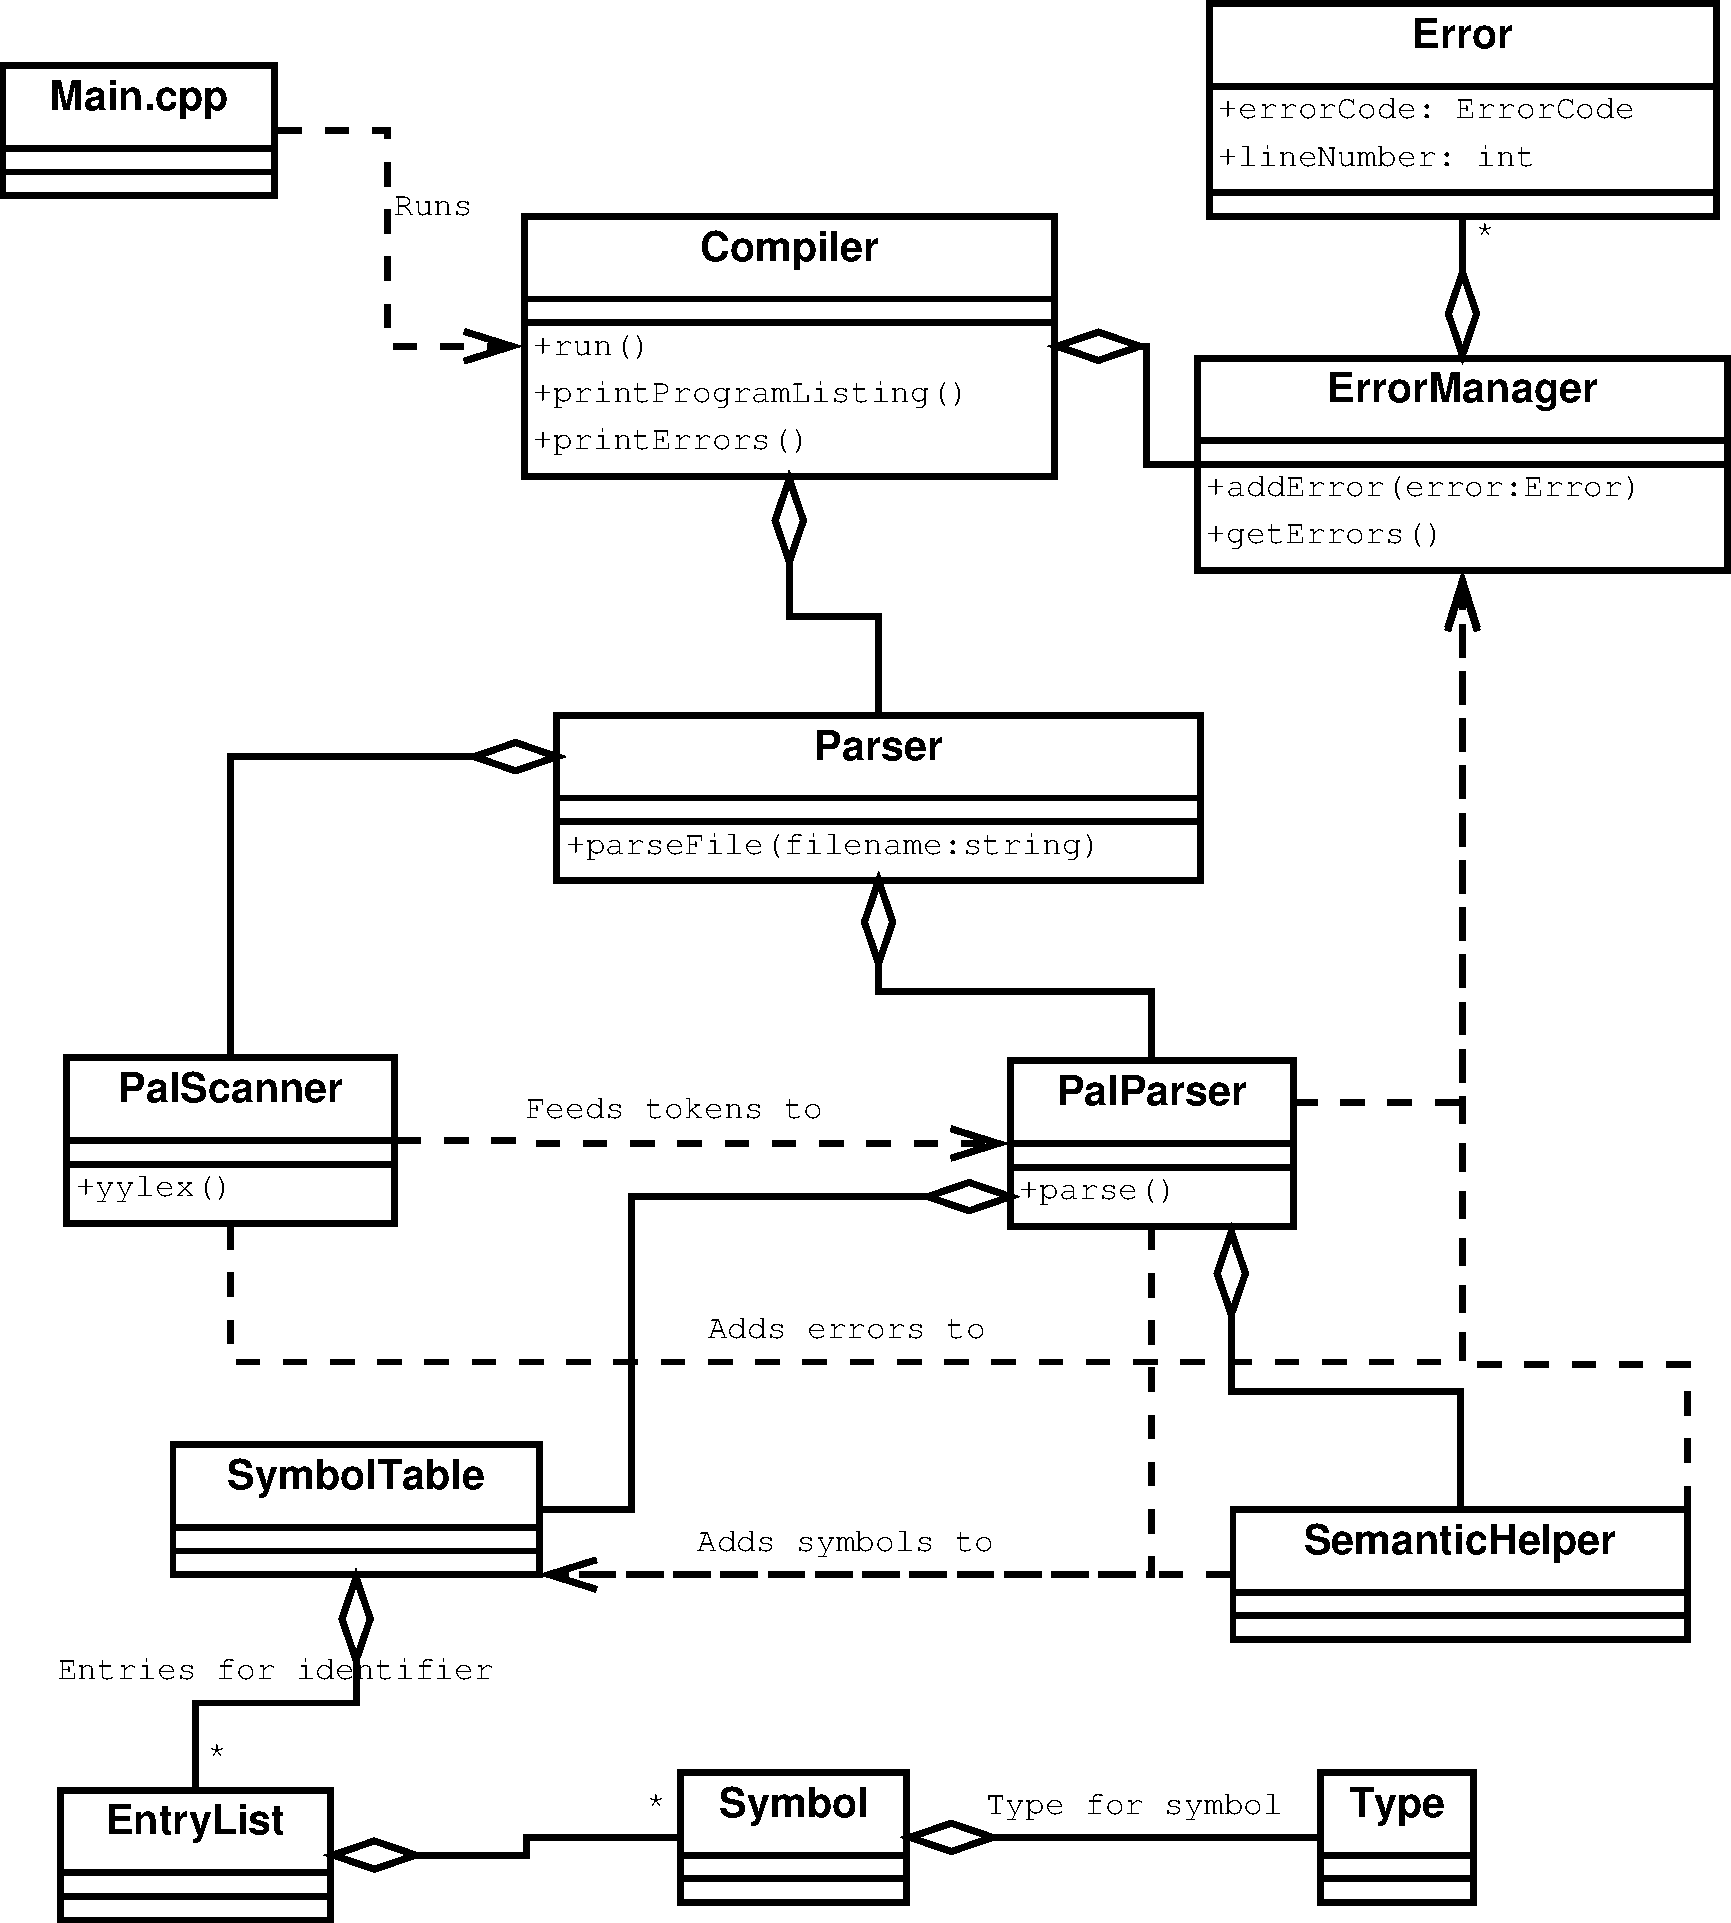
\includegraphics[width=10cm]{uml.pdf}
\caption{General structure of the compiler's parsing components.}
\end{figure}

At this stage, our compiler source consists of 6 classes. The \texttt{Compiler} class is instantiated by 
the program's \texttt{main()} function, and ran with the program's given command line arguments. 

The \texttt{Compiler} class creates an \texttt{ErrorManager}
class which tracks errors as they are detected while parsing the file. It passes the \texttt{ErrorManager}
to the \texttt{Parser} class when it is constructed.

The \texttt{Parser} class is a wrapper for the \texttt{flex} and \texttt{bison}
generated \texttt{PalScanner} and \texttt{PalParser} classes, from the
\texttt{pal.lex} and \texttt{pal.y} sources, respectively. \texttt{Parser}
parses a file with \texttt{parseFile(fileName)}, which creates a
\texttt{PalScanner} and \texttt{PalParser} where the scanner runs through
the file and feeds the parser with a stream of tokens.  The scanner and
parser are given access to the common \texttt{ErrorManager}, and when they
encounter errors during lexical and syntactical analysis, they create new
\texttt{Error} objects with the appropriate error code and line number and
give them to the \texttt{ErrorManager}.

When parsing is finished, the \texttt{Compiler} takes the errors accumulated by
the \texttt{ErrorManager} and either displays them inline with the program
listing, or all errors in order of appearance without the program listing if 
\texttt{pal} was invoked with the \texttt{-n} option.

	% Overall design
	% Outline of classes + dependencies

\section*{Lexical Analysis}

Our lexical analyser is generated by GNU Flex from the source in \texttt{./src/pal.lex}, which
is bundled into the \texttt{PalScanner} class. It is capable of recognizing the following
errors at the lexical level:

\begin{description}
  \item[Unclosed Comment]
	  If a comment is started with \texttt{\{} but is not followed by a
	  \texttt{\}} later in the file, the scanner will report an error.  In
	  our scanner, the comment rule will match to the end of the file in
	  this situation, so unfortunately no more analysis of the file is
	  possible at this point.
	  % TODO should we consider backtracking to the next line somehow?

  \item[Unexpected Comment End]
	  If the scanner encounters a \texttt{\}} when it is not in a comment,
	  it will report an error. Otherwise, the extra brace is ignored and analysis 
	  continues in an attempt to find more errors in the file.

  \item[Multi-line String Literal]
	  % TODO make sure this is actually implemented!
	  In the PAL language, a string literal cannot span multiple lines, so 
	  if the scanner encounters a string literal that extends beyond the next
	  newline, it will report an error that indicates the start and finish line
	  of the illegal multi-line string. It will still return a \texttt{STRING\_LITERAL}
	  token, and continue analysis to try and find more errors.

  \item[Invalid Character or Escaped Character in String]
	  The scanner will report an invalid character/escaped character in a string
	  literal if it contains either of the following:
	  \begin{itemize}
		  \item a \texttt{\textbackslash} that is not followed by a 
			  \texttt{'}, \texttt{n}, or \texttt{t}
		  \item a \texttt{\textbackslash} at the end of the string, that
			  is not preceded by another \texttt{\textbackslash}
	  \end{itemize}

	  % TODO would be cool if it actually printed the invalid character!

	% TODO \ at end of string? what kind of error? test!?

  \item[Invalid Identifier]
	  Valid PAL identifiers start with at least one letter, followed by any number
	  of letters or numbers. Identifiers that start with numbers will be reported
	  as an error. 
	% TODO can we detect other invalid identifiers?

  \item[Invalid character]
	  If the scanner detects an unknown character, such as \texttt{!} or
   \texttt{\#}, it returns an error indicating that an unrecognized
   character was found. It easily recovers from this error and
   continues on. 


\end{description}

\section*{Syntax Analysis}
Our syntax analyzer is generated by GNU Bison from the source in \texttt{./src/pal.ly}, which
is bundled into the \texttt{PalScanner} class. It is capable of recognizing the following
errors at the syntax level:

\begin{description}
  \item[Program Declarations]
	The compiler detects faults in the declaration. If it is missing a program
	will not compile. Errors will be outputted for the following cases:
		\begin{itemize}
			\item If the semicolon is missing
			\item If one or both arguments are missing
			\item If the program is missing a closing parentheses,
			starting, or both.
			\item If there is an invalid program name
		\end{itemize}
\item[Variable, Constant or Type Declarations]
	If a variable, constant or type is incorrectly declared, the compiler will
	catch the following errors:
		\begin{itemize}
			\item If an improper type of assignment is used. IE. 
			constant is declared using :, instead of = an appropriate
			error message will be emitted for each type.
			\item Improper variable names, only variables starting with
			a letter, and containing letters and numbers after are valid.
		\end{itemize}
		
\item[Enumerations]
	If an enumeration is incorrectly defined an error will be produced.
\item[Arrays]
	Arrays which are declared incorrectly, either by defining the set wrong, 
	or by specifying an invalid type will produce a specific error.
\item[Functions]	
	Functions will be checked for proper formatting if a function is invalid 
	an appropriate error will be emitted. Functions are required to have 
	return types, enclosing parameters and a ending semicolon. Each function 
	is required to have variables declared before the begin statement and required
	to be have a begin and end statement.
	
\item[Procedures]
	Procedures are declared in a similar fashion as functions, and have the same
	error checking except that they don't have a return value and are ended by 
	a period instead of a semicolon. 

\item[Expressions]
	Expressions will checked for proper structure. If a symbol is missing,
	semicolon or any part it will be discarded and return an error. 
	
\item[Recovery Strategies]
	Try to catch errors as early as possible by defining strict cases that are
	simple to implement but are common user errors. Errors which are not defined
	are given a generic error output, using the built in error within bison.

	% TODO
	% handling of lexical units
	% syntax error reporting
	% recovery strategies
\end{description}
\section*{Testing}
\begin{description}
	% TODO
	% gtest, unit tests
	% whole file tests
	
\item[GTest]
	For accurate tests of the compiler we used gtest. Within gtest we
	built specific tests using tokens. Our tests can be ran using,
	\texttt{\%make test}, \texttt{\%make ScannerTest}, or \texttt{\%make ParserTest}.
	(make test runs every test)
	\begin{itemize}
		\item \texttt{MockScanner.cpp} is a simple file. It defines a 
		'' MockScanner '', for use with testing. The Parser can be unit tested
		without the dependence of the real scanner which may contain errors.
		\item \texttt{ParserTest.cpp} contains a few tests which push
		tokens onto a stack and are fed to our parser to check if the 
		grammar contained in  \texttt{pal.y} is recognized correctly.
		
		\item \texttt{ScannerTest.cpp} Is used to check pal programs.
		By hand expected tokens are placed into this file, and if they match
		from the input file the test will pass.
		
		\item \texttt{ParserTestWithFiles.cpp} This file is automatically
		generated using a bash script. This file takes the tests in
		the test\_cases folder and builds a cpp file, if it is labeled vt*.pal
		the expected return is 0 (valid pal) or bt*.pal is 1 (invalid pal).
		This made it very easy to add test cases and to run them while making 
		changes to the grammar or token identifiers.
	\end{itemize}
\item[Submitted Tests 0.pal - 9.pal]
	Tests 0-4 contain 3 errors which are lexical. Tests 5-7 contain
	syntax errors, and tests 8 and 9 contain valid pal programs which 
	check tricky correct syntax. These tests are included at ''test\textbackslash 
	test\textunderscore cases\textbackslash checkpoint\textunderscore 1''.
\end{description}
% known bugs?
% extra features?

\end{document}
